\section{Using bounded model checking for coverage analysis of safety-critical software in an industrial setting \cite{angeletti2010}}

This paper proposes a new way of test case generation with the purpose of guaranteeing 100\% branch coverage. The way that constraint-based solving is used for test case generation
is based on symbolic execution, where path conditions are gathered and solved by a solver
to generate a series of possible input vectors. This approach usually fails on dealing with non-linearity, which makes it less practical for the industrial settings.
The idea of \cite{angeletti2010} is to use BMC for test case generation.
First, authors introduce a procedure for converting a subset of ANSI-C into a Boolean
formula in Conjunctive Normal Form w.r.t. a given depth for BMC. So, it means that loops are unwound according to the depth.

Here, there must be a specified property. Figure \ref{fig:testing-bmc} shows the process.
Program is seen by its control flow graph. To generate a test
that aims to cover a given block under test, the negation of the property
is added into the block, and then it is model checked. For model checking use the CBMC tool.
In other words, to generate a test that covers all the branches of a given function $f$,
the negation of the property is added to each basic block of $f$ as one new assertion at a time.
So, $f$ with $n$ basic blocks need $n$ runs of CMBC, and for each run the
depth of model checking may increase if needed. For each run, CMBC starts with depth $k = 1$,
then if it cannot find a counter example (test case), then $k$ is increased. Each time
that $k$ increases, a new code transformation and instrumentation is required.
The process stops when 100\% decision coverage is achieved.
To check that, a coverage analysis is performed using Cantata. if the
coverage score is not yet 100\% then $k$ is incremented
and test generation is repeated again.

\begin{figure}
  \centering
  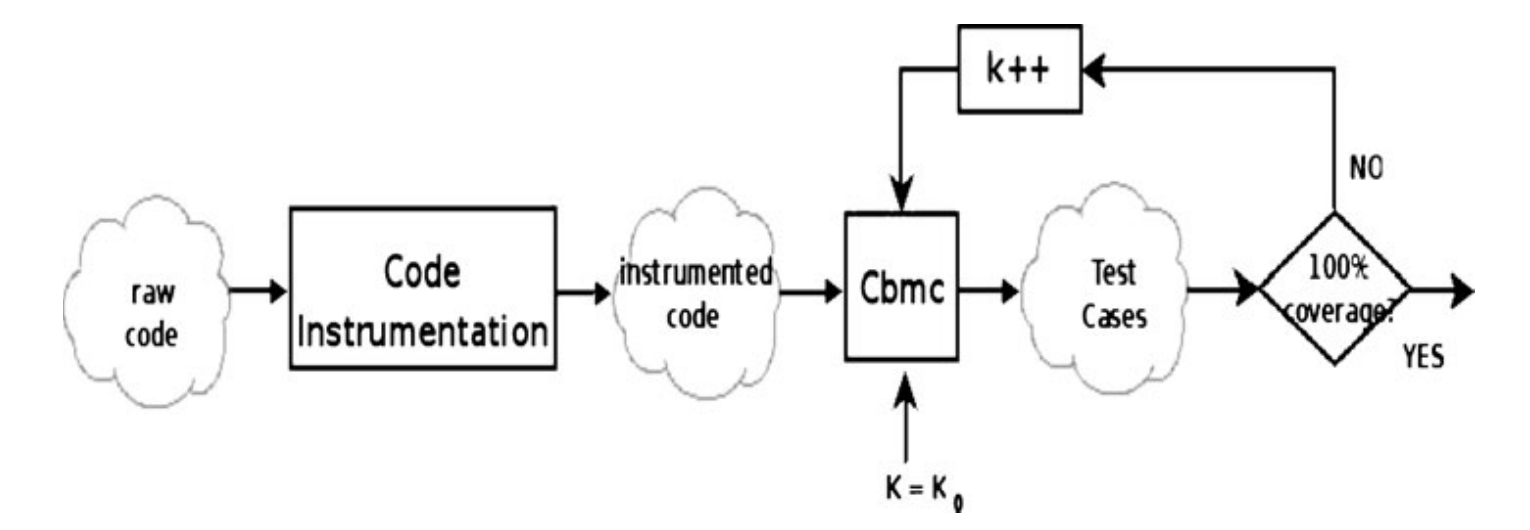
\includegraphics[width=\textwidth]{p1.png}
  \caption{process of testing with BMC}\label{fig:testing-bmc}
\end{figure}

They evaluated their method by an experiment on an industrial project, called EVC, with more than 100,000 lines of code. The experiment has been conducted on 5 modules of the project with 10,000 lines of code.  Then, the goal was to generate automatic
tests on the five modules of the EVC.
In terms of performance, results were compared
with manual test generation by a domain expert for 100\% coverage. The experimental results reports the idea is quite efficient and
can significantly reduce the testing effort.

\section{Convergence testing in term-level bounded model checking \cite{bryant2003convergence}}
They proposed a new way of formalizing convergence and
then a procedure for checking if BMC would converge or not.
The method for checking \emph{property}, to me, is the same as $k$-induction though.
They call it $k$-convergence. But, the goal of the paper is to \emph{determine whether a system is $k$-convergent for some
value of $k$}. They formulated ``convergence'' into second-order logic with quantifiers.
Then, since the problem is undecidable in general, they proposed two method for checking it:
(1) eliminating quantifiers and transform the formula into
first-order equations (then I'm not sure what method they used for verifying the new formula).
(2) they proposed an incomplete procedure to check their initial formulation in second-order logic (which I didn't get into its detail).
\linebreak
\linebreak
My questions:
\begin{itemize}
  \item is it practical?
  \item why do we need to formulate convergence?
  All we need to check is if the property is valid.
  So, I can think of ``convergence'' as a way of proving a property.
\end{itemize}

\section{Verification with small and short worlds \cite{sinha2012verification}}
Idea: Apply one-induction on the property, if it doesn't pass,
then compute an abstract model and verify the abstract model.
Obviously model can be abstracted in many different ways. After that, if property is valid on the abstract model, it means it will be valid on the original model. But, if property fails on abstraction, it could be either abstraction is not good enough, or property is not valid in general, which is the same initial problem we want to address with PDR, I think. We start with a very general model, then refine it in each frame w.r.t. the counterexample. Anyways, here the goal is not to refine the abstraction though. After abstraction, they  try  to  find  a  bound
$k$ on  the  reachability  diameter  of  the abstract model (or  small  world).
they call the BMC-checking of the small world the
``short world'' method, since it relies on computing a ``short''
bound  for  BMC.   The overall method is called ``Small-Short-World $(S^2W)$''.

The  main contribution is  a  set  of  heuristics  for  creating  an
abstract model and computing a bound on the reachability
diameter of its state space.

\emph{reachability diameter}: visiting all
reachable states, the minimum number of steps being the
reachability diameter
of the
model, or the longest path in the set of minimal paths to any reachable state.


\linebreak
\linebreak
My thoughts:
\begin{itemize}
  \item This is basically another verification method, which is to me pretty much similar to the idea behind PDR.
  \item But the interesting thing which could be helpful to me and I need to look at closely is
  the way bound $k$ is computed. If computing this bound or reachability diameter is easy, it could help us...
  \item is diameter different from $k$ when a property is $k$-inductive?

\end{itemize}


\section{Beyond vacuity: towards the strongest passing formula \cite{chockler2013beyond}}
Main reasons for a vacuous pass are possible errors in either the design or specification.
A specification $\phi$ is satisfied vacuously in $M$, if $M \vdash \phi$ and
there exists $\psi \subset \phi$ that does not affect $\phi$ in $M$.
Basically, vacuity check tries to
enumerate the useless literals of a specification (in contrary to IVCs;
IVCs show literals that are useful to the proof of the specification).

Mutual Vacuity: find the maximal set of literal occurrences that can be
replaced simultaneously with $false$ without falsifying the property in the model.

Goal of this paper: find a property stronger than $\phi$ that is still satisfied in $M$.
Among formulas satisfied by $M$, they want to find the strongest possible formula by
replacing literals in $\phi$ with $false$ and any Boolean combination of such formulas.
In other words, the goal is to compute a strong specification that is not vacuous.

First, they talk about vacuity/mutual vacuity and the fact that those king of definitions
don't suggest any ways of computing a strong specification.
\linebreak
\linebreak
my thoughts:
\begin{itemize}
  \item I think vacuity is more about the quality of the specification. And this paper wants to
  say that just knowing spec is vacuous or not is not enough. It would be cool to have the best (strongest) non-vacuous spec.
  \item what is this good for? why do we need to know the strongest? how does it help?
  \item this paper proposed for finite state systems with LTL properties
  \item I suspect practicality. What about performance?
  \item I think the method is more about collecting and trying out different possible specifications. However, vacuity could be because of design issues.
  \item With IVCs, we don't compute a strong specification, however that would be possible as well. When we do the vacuity check and a property is vacuous,
      we may be able to devise some way of computing strong and correct specification.
  \item my question: what is really a good specification? how can we quantify the quality of a specification? is it better for a specification to be strong or weak?!
      \item With completeness checking, we measure the overall quality of all properties.
      But, with vacuity checking, we can measure the quality of one property (in case we want to look at it in this way)

\end{itemize}

\subsection{Discussion with Mike over Coverage 9/20/2016}
\textbf{Difference between falsity coverage and vacuity coverage}
In falsity coverage, we mutate the design and see if the property is still valid or not.
In this way, we understand if that mutant was necessary (covered) for (by) that property.

There are couple of problems there that make us have the vacuity coverage:
\begin{enumerate}
  \item if the mutant shrinks the reachable state, the property will always be satisfied because
  in model checking property always holds of reachable states (and any subset of them).
  \item if the properties are vacuous then we get low coverage.
\end{enumerate}

In vacuity coverage, we know that all properties are non-vacuous (we checked them for vacuity). Then, we change (mutate)
the design. If the property is vacuous afterwards it means that the mutant was necessary for that property.
\linebreak
\linebreak
Summary:

falsity coverage: does the mutant FSM still satisfy the property?

vacuity coverage: if the mutant FSM still satisfies the property, does it satisfy it vacuously?

\section{Enhancing Symbolic Execution with Veritesting \cite{avgerinos2014}}


